\documentclass[12pt]{article}
\usepackage[hidelinks]{hyperref}    
\usepackage[all]{hypcap}
\usepackage{amssymb}
\usepackage{graphicx}
\graphicspath{{../images/}}
\title{\textbf{Analisi Matematica\\Nomenclatura e funzioni}}
\date{16 settembre 2024}
\author{Andrea Malvezzi}
\begin{document}
\maketitle
\pagebreak
\tableofcontents
\pagebreak
\section{Insiemi numerici}
\begin{itemize}
    \item $\mathbb{N} \rightarrow$ numeri naturali, \{$0$, $1$, $2$, $3$, $4$, ...\};
    \item $\mathbb{Z} \rightarrow$ numeri interi, \{..., $-2$, $-1$, $0$, $1$, $2$, ...\};
    \item $\mathbb{Q} \rightarrow$ numeri razionali, \{$\textit{p}/\textit{q}$ : \textit{p} $\in \mathbb{Z}$, \textit{q} $\in \mathbb{Z}$, \textit{q}$\neq 0$\};
    \item $\mathbb{R} \rightarrow$ numeri reali, \{..., -$\sqrt{5}$, $-1/2$, $0$, $1$, $4/7$, ...\}
\end{itemize}
\section{Notazioni}
\begin{itemize}
    \item $\in \rightarrow$ appartiene;
    \item $\notin \rightarrow$ non appartiene;
    \item $\forall \rightarrow$ per ogni;
    \item $":", "|" \rightarrow$ tale che;
    \item $\exists \rightarrow$ esiste (almeno uno);
    \item $\nexists \rightarrow$ non esiste;
    \item $\exists! \rightarrow$ esiste un unico elemento;
    \item $\lor \rightarrow$ vel/oppure, or logico;
    \item $\land \rightarrow$ et/e, and logico;
    \item $\subseteq \rightarrow$ inclusione tra insiemi;
    \item $\nsubseteq \rightarrow$ non inclusione tra insiemi;
    \item $\cup \rightarrow$ unione tra insiemi;
    \item $\cap \rightarrow$ intersezione tra insiemi;
\end{itemize}
\section{Implicazioni}
$\textit{p} \Rightarrow \textit{q}$:
\begin{itemize}
    \item $\textit{p} \rightarrow$ condizione \textbf{sufficiente} per far valere \textit{q} (\textbf{ipotesi});
    \item $\textit{q} \rightarrow$ condizione \textbf{necessaria} per far valere \textit{p} (\textbf{tesi});
\end{itemize}
\subsection{Esempio di implicazione}
\begin{itemize}
    \item $\textit{p} =$ "$x = 2$";
    \item $\textit{q} =$ "$x^2 = 4$";
    \item $\textit{p} \Rightarrow \textit{q} =$ "se \textit{p} ($x=2$) allora \textit{q} ($x^2=4$)";
\end{itemize}
Qui \textit{p} è condizione sufficiente per fare valere \textit{q}, in quanto $2^2=4$. Tuttavia, $2$ non è l'unica cifra per cui $x^2=4$, difatti anche $(-2)^2=4$.\\
D'altrocanto, per avere $x=2$ nel contesto della nostra implicazione \textbf{occorre} che \textit{q} valga. Quindi \textit{q} è condizione necessaria per fare valere \textit{p}.
\section{Negazioni}
Una negazione si indica con un "cappellino" sopra al simbolo che si vuole utilizzare:
\begin{itemize}
    \item $\not\forall$ che equivale a dire $\exists$;
    \item $\not\exists$ che equivale a dire $\forall$;
\end{itemize}
Inoltre, negare un'intera implicazione invertendo tesi e ipotesi mantiene la tabella di verità intoccata. Perciò:
\begin{itemize}
    \item $\not\textit{q} \Rightarrow \not\textit{p}$ è logicamente equivalente a $\textit{p} \Rightarrow \textit{q}$.
\end{itemize}
\section{Coimplicazioni}
\textit{p} $\Leftrightarrow$ \textit{q} $=$ \textit{p} \textbf{coimplica} \textit{q} oppure \textit{p} sse (se e solo se) \textit{q}.\\
Questo significa che:\\
\textit{p} $\Rightarrow$ \textit{q} $\land$ \textit{q} $\Rightarrow$ \textit{p}, ovvero che le proposizioni di \textit{p} e di \textit{q} sono logicamente equivalenti.
\subsection{Esempio di coimplicazione}
Consideriamo quanto segue:
\begin{itemize}
    \item \textit{p}: "Oggi è lunedì";
    \item \textit{q}: "Domani è martedì";
\end{itemize}
La coimplicazione \textit{p} $\Leftrightarrow$ \textit{q} si legge "Oggi è lunedì sse domani è martedì."\\
Quindi la coimplicazione varrà solamente nel caso in cui \textit{p} e \textit{q} siano entrambe vere o false contemporaneamente.
\section{Funzioni}
Una funzione definita da $A$ a $B$ si indica con la seguente scrittura:
\begin{center}
    $f:$ $A$ $\rightarrow$ $B$
\end{center}
Qui, $A$ corrisponde al \textbf{dominio} della funzione, mentre $B$ al suo \textbf{codominio}.
Tuttavia una funzione, per essere definita tale, deve rispettare la seguente \textbf{legge di associazione}:
\begin{center}
    $\forall a \in A, \exists! b \in B | f(a) = b$
\end{center}
Dove $b$ è detta immagine di $a$ tramite $f$.
\pagebreak
\subsection{Iniettività di una funzione (1-1)}
Una funzione si dice iniettiva quando vale il seguente:
\begin{center}
    $\forall a, a\textsubscript{1} \in A | a \not= a\textsubscript{1} \Rightarrow f(a) \not= f(a\textsubscript{1})$
\end{center}
L'iniettività di una funzione dipende strettamente dal dominio di questa. Certe volte è possibile rendere una funzione iniettiva riducendo il dominio e studiandone solamente una parte (vedi Tangente, etc...)
\subsubsection{Esempio di funzione NON iniettiva}
\begin{figure}[!htb]
    \centering
    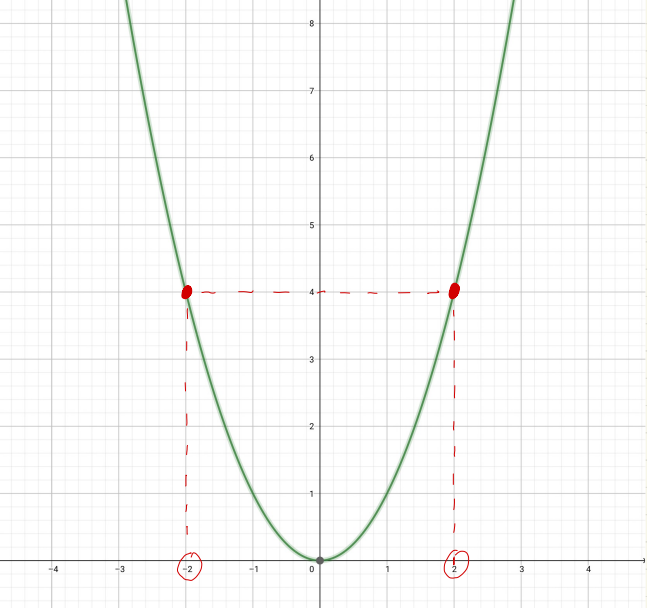
\includegraphics[width=.9\linewidth,height=.40\textheight,keepaspectratio]{lezione_1/iniet_func.png} % essenzialmente resiza l'immagine
    \begin{center}
        \caption{\label{fig:no_iniett_example}Un esempio di funzione NON iniettiva.} % label fuori da caption spesso non va, mettilo dentro
    \end{center}
\end{figure}
La funzione presentata NON è iniettiva in quanto $f(2) = f(-2)$.
\pagebreak
\subsection{Suriettività di una funzione (sv)}
Una funzione si dice suriettiva quando vale il seguente:
\begin{center}
    $\forall b \in B, \exists a \in A | f(a) = b$
\end{center}
La suriettività di una funzione definita nella maniera seguente:
\begin{center}
    f: $A$ $\rightarrow$ $B$
\end{center}
dipende strettamente dal codominio di $B$.
\subsubsection{Esempio di funzione NON suriettiva}
\begin{figure}[!htb]
    \centering
    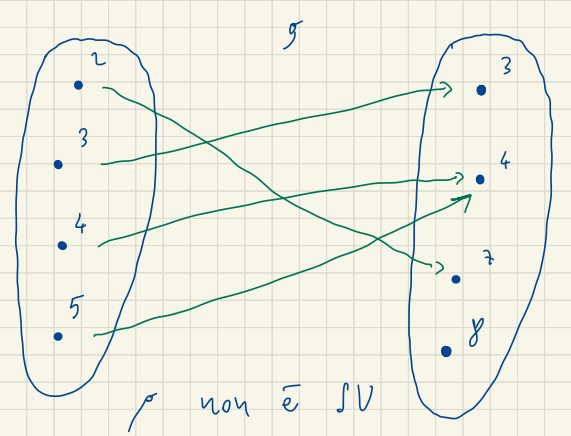
\includegraphics[width=.9\linewidth,height=.40\textheight,keepaspectratio]{lezione_1/sv_func.png} % essenzialmente resiza l'immagine
    \begin{center}
        \caption{\label{fig:no_sv_example}Un esempio di funzione NON suriettiva.} % label fuori da caption spesso non va, mettilo dentro
    \end{center}
\end{figure}
La funzione presentata non è suriettiva in quanto nel codominio della funzione l'8 non ha una corrispondenza con un numero del dominio di partenza.
\pagebreak
\end{document}